\chapter{基于任务反馈与协同增量重传的轻量化语义传输机制}
\label{chap:semantic}

\section{引言}

在端到端业务承载路径的可靠传输环节，资源受限的 LEO 卫星需要将采集图像传至地面，以支持场景分类等视觉任务。扩大星上语义编码器会增加卫星的计算、存储和能耗负担；生成式恢复模型虽可部署在地面，但其迭代推理仍会增加接收端处理时延和显存占用，不利于多轮反馈传输。LEO 图像传输还具有收发非对称性：卫星负责图像采集与编码，下游任务模型部署在地面。若发送端与具体任务绑定，卫星便需要随地面任务调整模型；若只进行一次开环传输，地面端难以根据当前任务判决确定后续增量传输的分块优先级。现有语义 HARQ 多返回确认信息或标量质量信息，难以提供分块级的任务判决敏感度。跨轮接收采用固定平均或直接替换时，还可能覆盖历史语义状态中保留的分块表征。

为解决上述问题，本章提出面向收发资源非对称 LEO 图像传输的接收端驱动协同增量语义重传（Coordinated Incremental Semantic Retransmission，CIS-R）机制，构建“地面任务判决—分块级反馈—星上选择性增量传输—地面跨轮状态累积”闭环。地面接收端利用当前判决裕量对分块级接收表征的局部敏感度生成 Top-$K$ 反馈掩码；星上发送端依据反馈与轮次信息生成候选增量，并仅打包传输请求分块；地面接收端通过掩码引导的门控累积更新所选分块并保留其余分块的历史状态。在线传输阶段，星上发送端无需部署或访问下游任务模型、任务输出和任务标签，任务模型推理、分块优先级计算与反馈生成均由地面接收端完成。ImageNet-100 仿真与轨迹驱动星地链路实验在所测试条件下验证了任务驱动分块选择和跨轮累积的有效性，并分别统计星上发送端与地面接收端的实现级开销。本章相关成果已撰写成会议论文 ``CIS-R: Receiver-Driven Incremental Semantic Retransmission for Resource-Constrained LEO Image Delivery''，投稿于 IEEE International Conference on Computer Communications（INFOCOM）2027。

\section{系统模型与问题建模}
\label{sec:ch6_sysmodel}

考虑由资源受限 LEO 卫星和地面接收端组成的非对称图像传输系统。星上发送端承担图像采集、基础语义编码与补充信道表征生成，地面接收端部署语义解码器、下游任务模型、分块优先级计算和接收状态累积模块。在线传输期间，星上发送端仅使用源图像分块、反馈掩码和轮次信息，不访问任务模型参数、任务输出或任务标签。每幅图像执行一轮基础传输和预设的 $R$ 轮增量传输，接收端在每个增量轮开始前依据当前接收状态重新计算分块优先级。

本节主要符号汇总如表~\ref{tab:ch6_symbols} 所示。

\begin{longtable}[c]{@{}p{0.21\textwidth}p{0.245\textwidth}p{0.21\textwidth}p{0.245\textwidth}@{}}
\bicaption{CIS-R 系统模型主要符号汇总}{Main notation used in the system model of CIS-R}
\label{tab:ch6_symbols} \\
\toprule
符号 & 含义 & 符号 & 含义 \\
\midrule
\endfirsthead
\multicolumn{4}{l}{\textbf{续表~\thetable}} \\
\toprule
符号 & 含义 & 符号 & 含义 \\
\midrule
\endhead
\midrule
\multicolumn{4}{r}{续下页} \\
\endfoot
\bottomrule
\endlastfoot
  $\mathbf X,\ H,\ W,\ C_{\mathrm{img}}$ & 源图像、图像高、图像宽与图像通道数 & $f_{\mathrm{pat}},\ f_{\mathrm{unpat}}$ & 图像分块映射与反分块映射 \\
  $\mathbf P,\ \mathbf p_n,\ N,\ D$ & 分块特征序列、单分块特征、分块数与分块特征维度 & $\mathbf Y^{(r)},\ \mathbf y_n^{(r)}$ & 第 $r$ 轮分块级接收表征（语义状态）与第 $n$ 个分块表征 \\
  $\mathcal T_\phi,\ \hat{\mathbf X}^{(r)},\ \mathbf l^{(r)},\ \Delta^{(r)}$ & 冻结的接收端任务模型、恢复图像表征、任务输出向量与判决裕量 & $r,\ R,\ \mathbf e_r$ & 传输轮次、最大增量重传轮数与轮次嵌入 \\
  $f_{\mathrm{base}},\ \mathrm{Norm},\ g_{\mathrm{dec}}$ & 基础编码器、平均功率归一化与语义解码器 & $\mathbf Z^{(0)},\ \hat{\mathbf Z}^{(0)}$ & 基础传输负载与相应接收负载 \\
  $\mathbf M_{\mathrm{hard}}^{(r)},\ K,\ \mathcal I^{(r)}$ & 第 $r$ 轮二进制反馈掩码、选定分块数与分块索引集合 & $\mathcal F_{\mathrm{tx}},\ \tilde{\mathbf Z}^{(r)}$ & 反馈与轮次条件化增量生成映射及候选补充信道表征 \\
  $\operatorname{Pack},\ \mathbf Z^{(r)}$ & 所选分块打包操作与第 $r$ 轮归一化发送负载 & $\hat{\mathbf Z}^{(r)},\ \mathbf N^{(r)},\ \sigma_r^2$ & 第 $r$ 轮接收负载、AWGN 噪声与噪声方差 \\
  $\hat{\mathbf Z}_{\mathrm{full}}^{(r)},\ \operatorname{Scatter},\ \tilde{\mathbf U}^{(r)}$ & 零填充信道表征、索引回填操作与完整解码表征 & $\bar{\mathbf M}_{\mathrm{hard}}^{(r)},\ \mathbf U^{(r)},\ \mathbf G^{(r)},\ \tilde{\mathbf Y}^{(r)}$ & 特征维广播掩码、本轮补充语义特征、融合门与候选融合状态 \\
  $\rho_r,\ D_r$ & 第 $r$ 轮信噪比与发送负载实值维数 & $d(t_r),\ c,\ \tau_{\mathrm{prop}}^{(r)}$ & 星地斜距、光速与单向传播时延 \\
  $\epsilon,\ L^{(0)},\ L^{(r)}$ & 单分块实值信道维数、基础轮与增量轮信道使用次数 & $\mathrm{CBR}^{(r)},\ B_{\mathrm{fb}}^{(r)}$ & 累积信道带宽比与累积反馈比特数 \\
\end{longtable}

\noindent(1)~\textbf{非对称 LEO 图像传输场景}

记星上发送端采集的源图像为 $\mathbf X\in\mathbb R^{H\times W\times C_{\mathrm{img}}}$，其中 $H$、$W$ 与 $C_{\mathrm{img}}$ 分别表示图像高度、宽度和通道数。分块映射将源图像转换为
\begin{equation}\label{eq:ch6_patch}
\mathbf P=f_{\mathrm{pat}}(\mathbf X)
=\begin{bmatrix}
\mathbf p_1^{\mathsf T}\\[-1pt]
\vdots\\[-1pt]
\mathbf p_N^{\mathsf T}
\end{bmatrix}
\in\mathbb R^{N\times D},\qquad \mathbf p_n\in\mathbb R^{D},
\end{equation}
其中，$N$ 为图像分块数，$D$ 为单个分块的特征维度。

第 $r$ 轮传输结束后，地面接收端维护分块级接收表征
\begin{equation}\label{eq:ch6_state}
\mathbf Y^{(r)}
=\begin{bmatrix}
(\mathbf y_1^{(r)})^{\mathsf T}\\[-1pt]
\vdots\\[-1pt]
(\mathbf y_N^{(r)})^{\mathsf T}
\end{bmatrix}
\in\mathbb R^{N\times D}.
\end{equation}
本文将其称为第 $r$ 轮语义状态。该表征可通过反分块映射重构为图像域表征 $\hat{\mathbf X}^{(r)}=f_{\mathrm{unpat}}(\mathbf Y^{(r)})$。冻结的接收端任务模型输出
\begin{equation}\label{eq:ch6_logits}
\mathbf l^{(r)}=\mathcal T_\phi\!\left(\hat{\mathbf X}^{(r)}\right),
\end{equation}
其中，$\mathbf l^{(r)}$ 为任务输出向量。接收端依据该向量评估当前分块级接收表征，并生成下一轮分块反馈。

\noindent(2)~\textbf{多轮语义增量重传模型}

协同增量语义重传（Coordinated Incremental Semantic Retransmission，CIS-R）包括一轮基础传输和至多 $R$ 轮接收端驱动的增量重传。记传输轮次为 $r\in\{0,1,\dots,R\}$，其中 $r=0$ 表示基础传输。星上发送端首先生成
\begin{equation}\label{eq:ch6_base}
\mathbf Z^{(0)}=\mathrm{Norm}\!\left(f_{\mathrm{base}}(\mathbf P)\right)
\in\mathbb R^{N\times\epsilon},
\end{equation}
其中，$f_{\mathrm{base}}(\cdot)$ 为基础编码器，$\epsilon$ 为单分块实值信道维数。对于包含 $D_A$ 个实值传输维数的任意发送张量 $\mathbf A$，平均功率归一化定义为
\begin{equation}\label{eq:ch6_norm}
\mathrm{Norm}(\mathbf A)=\sqrt{\frac{D_A}{\lVert\mathbf A\rVert_2^2}}\,\mathbf A,
\qquad
\frac{1}{D_A}\left\lVert\mathrm{Norm}(\mathbf A)\right\rVert_2^2=1.
\end{equation}
基础负载经过前向信道后记为 $\hat{\mathbf Z}^{(0)}$，地面接收端将其解码为基础分块级接收表征 $\mathbf Y^{(0)}=g_{\mathrm{dec}}(\hat{\mathbf Z}^{(0)})\in\mathbb R^{N\times D}$。$\mathbf Y^{(0)}$ 不依赖具体下游任务，并作为后续增量重传的初始语义状态。

对任意增量重传轮 $r\geq1$，接收端生成二进制掩码 $\mathbf M_{\mathrm{hard}}^{(r)}\in\{0,1\}^{N}$，并满足 $\lVert\mathbf M_{\mathrm{hard}}^{(r)}\rVert_0=K$。该掩码指示本轮请求的 $K$ 个图像分块。星上发送端根据源分块特征、反馈掩码和轮次嵌入，为全部 $N$ 个分块生成候选补充信道表征
\begin{equation}
\tilde{\mathbf Z}^{(r)}=\mathcal F_{\mathrm{tx}}\!\left(\mathbf P,\mathbf M_{\mathrm{hard}}^{(r)},\mathbf e_r\right)
\in\mathbb R^{N\times\epsilon}.
\end{equation}
定义所选分块的有序索引集合为 $\mathcal I^{(r)}=\{n:M_{\mathrm{hard},n}^{(r)}=1\}$。实际送入物理信道的负载仅包含这些分块：
\begin{equation}\label{eq:ch6_maskinc}
\begin{aligned}
\mathbf Z^{(r)}
&=\mathrm{Norm}\!\left(
\operatorname{Pack}\!\left(\tilde{\mathbf Z}^{(r)},\mathcal I^{(r)}\right)
\right)\\
&=\mathrm{Norm}\!\left(
\left[\tilde{\mathbf z}_{n}^{(r)}\right]_{n\in\mathcal I^{(r)}}
\right)
\in\mathbb R^{K\times\epsilon},\qquad r\geq1.
\end{aligned}
\end{equation}
基础轮用于建立初始分块级接收表征，增量轮仅传输接收端请求的 $K$ 个分块。接收端仅更新反馈掩码选中的分块，其余分块沿用上一轮的接收状态。具体的接收状态更新过程将在第~\ref{subsec:ch6_accum}~节给出。

\noindent(3)~\textbf{AWGN 前向链路与低开销反馈链路}

各轮语义负载通过加性白高斯噪声（Additive White Gaussian Noise，AWGN）前向链路传输。由式~\eqref{eq:ch6_norm}，基础负载和增量负载均满足单位平均发送功率约束。记第 $r$ 轮发送负载包含的实值信道维数为 $D_r$，其中 $D_0=N\epsilon$，$D_r=K\epsilon$（$r\geq1$），则第 $r$ 轮信道模型及噪声分布写为
\begin{equation}\label{eq:ch6_channel}
\begin{aligned}
\hat{\mathbf Z}^{(r)}&=\mathbf Z^{(r)}+\mathbf N^{(r)},\\
\operatorname{vec}\!\left(\mathbf N^{(r)}\right)
&\sim\mathcal N\!\left(\mathbf 0_{D_r},\sigma_r^2\mathbf I_{D_r}\right),
\qquad \sigma_r^2=10^{-\rho_r/10}.
\end{aligned}
\end{equation}
其中，$\rho_r$ 为第 $r$ 轮接收信噪比（单位为 dB），不同轮次的 AWGN 相互独立。静态仿真在一次训练和测试中采用固定 SNR。时变链路仿真在每轮开始时读取当前 $\rho_r$，并获取时刻 $t_r$ 的星地斜距 $d(t_r)$。相应的单向传播时延为
\begin{equation}
\tau_{\mathrm{prop}}^{(r)}=\frac{d(t_r)}{c},
\end{equation}
其中，$c$ 为光速。

反向链路仅传输二进制掩码 $\mathbf M_{\mathrm{hard}}^{(r)}$，并假定该掩码由可靠的低速率控制链路承载。每轮反馈固定占用 $N$ bit。对于 $14\times14$ 分块网格，单轮反馈量为 $196$ bit，三轮增量重传的累计反馈量为 $588$ bit。反馈中不携带高维语义特征、任务模型参数或任务输出，星上发送端只解析分块选择信息。

\noindent(4)~\textbf{通信开销与受限传输问题建模}

记每个发送分块占用 $\epsilon$ 个实值信道维数，并按两个实值维数对应一次复信道使用计数。基础轮与单个增量重传轮的前向负载分别为
\begin{equation}\label{eq:ch6_round_payloads}
L^{(0)}=\frac{N\epsilon}{2},\qquad
L^{(r)}=\frac{K\epsilon}{2},\quad r\geq1.
\end{equation}
截至第 $r$ 轮的累积信道带宽比（Channel Bandwidth Ratio，CBR）为
\begin{equation}\label{eq:ch6_cbr}
\mathrm{CBR}^{(r)}=\frac{\epsilon(N+rK)}{2HWC_{\mathrm{img}}},
\qquad r\in\{0,\ldots,R\}.
\end{equation}
反向链路累计开销单独记为
\begin{equation}
B_{\mathrm{fb}}^{(r)}=rN\quad\text{bit}.
\end{equation}
在上述模型中，$K$ 给出每轮请求的分块数量，$\epsilon$ 规定每个分块的前向负载，$R$ 限制增量重传次数。本章研究的问题是：在给定前向传输预算、反馈开销和最大重传轮数的条件下，如何利用接收端任务反馈确定增量传输的分块优先级，并通过跨轮累积提高地面接收端的任务性能。

\section{接收端驱动的协同增量语义重传框架设计}
\label{sec:ch6_framework}

协同增量语义重传（Coordinated Incremental Semantic Retransmission，CIS-R）由决策敏感分块优先级评估、反馈条件化候选增量生成与选择性传输、掩码引导的增量语义累积三个模块构成。分块优先级评估将接收端当前判决对分块级接收表征的局部敏感度转换为后续传输优先级；反馈条件化候选增量生成以分块是否入选及当前轮次为条件生成补充信道表征，并依据 Top-$K$ 索引仅打包传输入选分块；掩码引导的门控累积限定接收状态的更新位置，并在所选分块上自适应融合历史表征与当前增量。三个模块共同形成接收状态更新驱动下一轮分块选择的闭环，使任务性能增益来自增量通信而非星上模型规模扩展。

\begin{figure}[!htp]
    \centering
    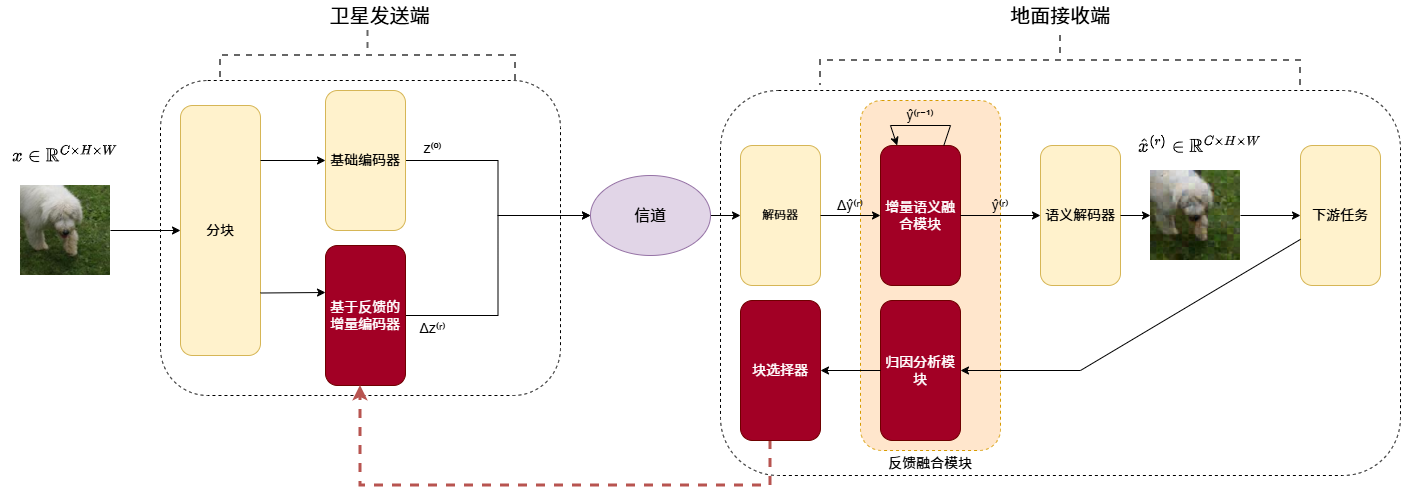
\includegraphics[width=\linewidth]{figures/chapter6/figs/system_model.png}
    \bicaption{接收端驱动的 CIS-R 语义重传框架}{Receiver-driven semantic retransmission framework of CIS-R}
    \label{fig:ch6_system_model}
\end{figure}

\subsection{框架总览}
\label{subsec:ch6_protocol}

图~\ref{fig:ch6_system_model} 给出了 CIS-R 的非对称收发结构。星上发送端包括分块映射 $f_{\mathrm{pat}}$、基础编码器 $f_{\mathrm{base}}$ 和轻量反馈条件化增量生成模块 $\mathcal F_{\mathrm{tx}}$；地面接收端包括语义解码器 $g_{\mathrm{dec}}$、增量累积模块 $\mathcal F_{\mathrm{rx}}$、冻结的任务模型 $\mathcal T_\phi$ 和反馈生成模块 $\mathcal F_{\mathrm{mask}}$。前向链路承载基础负载和增量负载，反向控制链路仅承载分块掩码。地面接收端在每次状态更新后重新生成分块掩码，星上发送端利用该掩码确定下一轮前向负载，地面接收端再利用同一掩码约束相应轮次的状态更新位置，从而形成由接收状态演化驱动后续选择性增量传输的闭环。

算法~\ref{algo:ch6_cis} 给出了上述实体之间的多轮收发顺序。

\begin{algorithm}[!htp]
\caption{接收端驱动的协同增量语义重传（CIS-R）收发流程}
\label{algo:ch6_cis}
\KwIn{星上源图像 $\mathbf X$，最大增量重传轮数 $R$，每轮选择分块数 $K$，相邻轮次重复选择抑制因子 $\eta$；地面端持有的冻结任务模型 $\mathcal T_\phi$}
\KwOut{完成第 $R$ 轮增量重传后的任务输出}
发送端计算分块特征 $\mathbf P=f_{\mathrm{pat}}(\mathbf X)$\;
发送端生成基础负载 $\mathbf Z^{(0)}=\mathrm{Norm}(f_{\mathrm{base}}(\mathbf P))$，并按式~\eqref{eq:ch6_channel} 经前向链路发送\;
接收端解码基础分块级接收表征 $\mathbf Y^{(0)}=g_{\mathrm{dec}}(\hat{\mathbf Z}^{(0)})$\;
\For{$r\leftarrow 1$ \KwTo $R$}{
  接收端计算 $\mathbf l^{(r-1)}=\mathcal T_\phi(f_{\mathrm{unpat}}(\mathbf Y^{(r-1)}))$\;
  接收端按照式~\eqref{eq:ch6_margin}--\eqref{eq:ch6_penalty} 计算判决裕量和分块优先级\;
  接收端选取 Top-$K$ 分块生成 $\mathbf M_{\mathrm{hard}}^{(r)}$，并经反向链路回传；发送端据此确定 $\mathcal I^{(r)}$\;
  发送端生成全部分块的候选补充信道表征 $\tilde{\mathbf Z}^{(r)}=\mathcal F_{\mathrm{tx}}(\mathbf P,\mathbf M_{\mathrm{hard}}^{(r)},\mathbf e_r)$\;
  发送端按式~\eqref{eq:ch6_maskinc} 打包并归一化 $\mathcal I^{(r)}$ 对应的分块，再按式~\eqref{eq:ch6_channel} 发送 $\mathbf Z^{(r)}$\;
  接收端按照式~\eqref{eq:ch6_increment_scatter}--\eqref{eq:ch6_increment_mask} 回填接收信道表征，解码后利用硬掩码提取本轮补充语义特征 $\mathbf U^{(r)}$\;
  接收端按式~\eqref{eq:ch6_accum} 更新分块级接收表征 $\mathbf Y^{(r)}$\;
}
接收端输出 $\mathcal T_\phi(f_{\mathrm{unpat}}(\mathbf Y^{(R)}))$\;
\end{algorithm}

\subsection{任务驱动的决策敏感分块优先级评估}
\label{subsec:ch6_feedback}

第 $r$ 轮增量重传开始前，地面端根据当前任务判决对图像分块排序。由语义状态 $\mathbf Y^{(r-1)}$ 恢复图像表征 $\hat{\mathbf X}^{(r-1)}=f_{\mathrm{unpat}}(\mathbf Y^{(r-1)})$ 后，任务模型输出 $\mathbf l^{(r-1)}=\mathcal T_\phi(\hat{\mathbf X}^{(r-1)})$。对于分类任务，将最大任务输出与次大任务输出之差定义为判决裕量：
\begin{equation}\label{eq:ch6_margin}
\Delta^{(r-1)}=l_{(1)}^{(r-1)}-l_{(2)}^{(r-1)}.
\end{equation}
其中，$l_{(1)}^{(r-1)}$ 和 $l_{(2)}^{(r-1)}$ 分别是 $\mathbf l^{(r-1)}$ 中的最大值和次大值。判决裕量对分块级接收表征的梯度用于衡量当前任务输出对该分块表征的局部敏感度。任务模型参数保持冻结，但接收端仍可计算任务输出关于输入表征的梯度 $\partial \Delta^{(r-1)}/\partial\mathbf Y^{(r-1)}$，用于分块敏感度评估。

第 $n$ 个分块的优先级还与其当前特征幅度有关。为此，将梯度与特征激活相乘，得到分块归因评分
\begin{equation}\label{eq:ch6_attr}
C_n^{(r)}=\sum_{d=1}^{D}\left|\frac{\partial \Delta^{(r-1)}}{\partial Y_{n,d}^{(r-1)}}\,Y_{n,d}^{(r-1)}\right|.
\end{equation}
$C_n^{(r)}$ 越大，说明第 $n$ 个分块表征对当前任务判决的局部影响越大，增量重传时具有更高的选择优先级。该评分仅用于分块间的相对排序，不等同于信息缺失判定或重传后的准确率增益预测。

将归因评分进行最小--最大归一化，结果记为 $V_n^{(r)}$。若某个分块在相邻轮次连续入选，有限的增量传输资源可能过度集中于同一位置。因此，从第二轮增量重传开始，降低上一轮已选分块的评分：
\begin{equation}\label{eq:ch6_penalty}
\bar V_n^{(r)}=
\begin{cases}
\eta\,V_n^{(r)}, & M_{\mathrm{hard},n}^{(r-1)}=1,\\[2pt]
V_n^{(r)}, & M_{\mathrm{hard},n}^{(r-1)}=0,
\end{cases}
\quad r\ge2,
\end{equation}
其中，$\bar V_n^{(1)}=V_n^{(1)}$，$\eta\in[0,1]$ 为相邻轮次重复选择抑制因子。该处理只下调上一轮被选择分块的当前评分，不对更早轮次的选择历史累计施加惩罚，并仍允许对当前任务判决持续敏感的分块再次入选。接收端从 $\bar{\mathbf V}^{(r)}$ 中选取评分最高的 $K$ 个分块，生成 $\mathbf M_{\mathrm{hard}}^{(r)}$。反向链路只需传输这一二进制掩码。

\subsection{反馈条件化候选增量生成与选择性传输}
\label{subsec:ch6_refine}

CIS-R 采用空间特征变换（Spatial Feature Transform，SFT），以单个分块的二值入选状态和轮次嵌入作为条件。第 $n$ 个分块的条件向量为 $\mathbf c_n^{(r)}=[M_{\mathrm{hard},n}^{(r)},\mathbf e_r]$，相应的缩放参数与平移参数满足
\begin{equation}
[\boldsymbol\gamma_n^{(r)},\boldsymbol\beta_n^{(r)}]
=f_{\mathrm{SFT}}(\mathbf c_n^{(r)}).
\end{equation}
SFT 对原始分块特征的调制结果为
\begin{equation}\label{eq:ch6_sft}
\mathbf p_{n,\mathrm{mod}}^{(r)}=\boldsymbol\gamma_n^{(r)}\odot\mathbf p_n+\boldsymbol\beta_n^{(r)},
\end{equation}
其中，$\boldsymbol\gamma_n^{(r)}$ 与 $\boldsymbol\beta_n^{(r)}$ 分别为第 $n$ 个分块的缩放参数和平移参数。调制后的特征送入轻量残差增量网络：
\begin{equation}
\tilde{\mathbf z}_n^{(r)}=f_{\mathrm{res}}\!\left(\mathbf p_{n,\mathrm{mod}}^{(r)}\right)
\in\mathbb R^{\epsilon}.
\end{equation}
式~\eqref{eq:ch6_sft} 对 $n=1,\ldots,N$ 均执行一次。反馈掩码以每个分块的二值选择状态参与编码映射，并确定实际发送集合；轮次嵌入使该条件映射随增量传输轮次变化。各分块的补充信道表征由源分块特征 $\mathbf p_n$ 与上述条件共同生成。

发送端按照反馈掩码形成索引集合 $\mathcal I^{(r)}$，并依据式~\eqref{eq:ch6_maskinc} 从 $N$ 个候选表征中打包接收端请求的 $K$ 个分块。星上计算覆盖全部 $N$ 个分块，前向链路仅承载其中 $K$ 个分块；相应的信道占用由 $K$ 和单分块实值信道维数 $\epsilon$ 决定。

\subsection{掩码引导的增量语义累积}
\label{subsec:ch6_accum}

接收端首先将本轮接收的 $K$ 个有效分块表征按照反馈索引回填至 $N\times\epsilon$ 的零填充信道表征，再输入与基础轮共享参数的语义解码器。解码器输出完整的 $N\times D$ 分块表征后，硬掩码仅保留本轮被请求位置的解码结果，其余位置置零并在后续融合中保持历史状态不变。具体地，$\hat{\mathbf Z}^{(r)}\in\mathbb R^{K\times\epsilon}$ 表示本轮接收的有效分块信道表征，回填操作写为
\begin{equation}\label{eq:ch6_increment_scatter}
\hat{\mathbf Z}_{\mathrm{full}}^{(r)}
:=\operatorname{Scatter}\!\left(
\hat{\mathbf Z}^{(r)},\mathcal I^{(r)},N
\right)
\in\mathbb R^{N\times\epsilon},
\end{equation}
其中，$\operatorname{Scatter}(\cdot)$ 将 $\mathcal I^{(r)}$ 指定位置之外的信道表征置零。共享语义解码器据此输出完整分块表征
\begin{equation}\label{eq:ch6_increment_decode}
\tilde{\mathbf U}^{(r)}
:=g_{\mathrm{dec}}\!\left(\hat{\mathbf Z}_{\mathrm{full}}^{(r)}\right)
\in\mathbb R^{N\times D}.
\end{equation}
为使分块掩码与特征矩阵维度一致，定义沿特征维复制后的掩码为
\begin{equation}\label{eq:ch6_mask_broadcast}
\bar{\mathbf M}_{\mathrm{hard}}^{(r)}
=\mathbf M_{\mathrm{hard}}^{(r)}\mathbf 1_D^{\mathsf T}
\in\{0,1\}^{N\times D},
\end{equation}
并利用硬掩码提取本轮补充语义特征
\begin{equation}\label{eq:ch6_increment_mask}
\mathbf U^{(r)}
:=\bar{\mathbf M}_{\mathrm{hard}}^{(r)}\odot\tilde{\mathbf U}^{(r)}
\in\mathbb R^{N\times D}.
\end{equation}
其中，$\mathbf 1_D$ 为 $D$ 维全一列向量，$\mathbf 1_{N\times D}$ 为 $N\times D$ 维全一矩阵。此时，$\mathbf Y^{(r-1)}$、$\mathbf U^{(r)}$ 和 $\mathbf G^{(r)}$ 均属于 $\mathbb R^{N\times D}$。历史分块级接收表征仍包含有效信息，当前增量各特征维的可靠性也不完全相同。CIS-R 根据二者联合生成融合门：
\begin{equation}\label{eq:ch6_accum}
\begin{aligned}
\mathbf G^{(r)}&=\sigma\!\left(f_g\!\left([\mathbf Y^{(r-1)},\mathbf U^{(r)}]\right)\right),\\
\tilde{\mathbf Y}^{(r)}&=\mathbf G^{(r)}\odot\mathbf Y^{(r-1)}+\left(1-\mathbf G^{(r)}\right)\odot\mathbf U^{(r)},\\
\mathbf Y^{(r)}&=\bar{\mathbf M}_{\mathrm{hard}}^{(r)}\odot\tilde{\mathbf Y}^{(r)}
+\left(\mathbf 1_{N\times D}-\bar{\mathbf M}_{\mathrm{hard}}^{(r)}\right)\odot\mathbf Y^{(r-1)},
\end{aligned}
\end{equation}
其中，$f_g(\cdot)$ 为融合门生成网络，$\sigma(\cdot)$ 为 sigmoid 函数。对于被请求的分块，$\mathbf G^{(r)}$ 逐维调节历史状态与当前增量的融合比例；其余分块不参与本轮更新，继续沿用 $\mathbf Y^{(r-1)}$ 中的状态。

\subsection{两阶段训练目标}
\label{subsec:ch6_train}

第一阶段训练任务无关的基础传输模块。分块映射、基础编码器、语义解码器和反分块映射采用图像重建损失联合训练：
\begin{equation}\label{eq:ch6_base_loss}
\mathcal L_{\mathrm{base}}
=\left\|f_{\mathrm{unpat}}\!\left(g_{\mathrm{dec}}(\hat{\mathbf Z}^{(0)})\right)-\mathbf X\right\|_2^2.
\end{equation}
这一阶段不使用下游任务模型，训练得到的基础语义状态作为地面端后续任务处理和增量累积的初始输入。

第二阶段进行离线任务监督训练。该阶段冻结基础传输模块和任务模型参数，只训练 SFT 参数生成网络、残差增量网络和接收端融合门。分类任务在第 $r$ 轮采用交叉熵损失 $\mathcal L_{\mathrm{task}}^{(r)}=\mathrm{CE}(\mathbf l^{(r)},y)$。任务模型参数虽不更新，但损失梯度仍可通过任务模型传至输入分块级接收表征，用于更新增量生成模块和接收端融合门。任务标签、任务模型推理及梯度计算均位于地面训练平台；在线传输阶段的星上发送端根据源图像、反馈掩码和轮次信息生成候选补充信道表征，再依据反馈索引打包本轮前向传输分块。为抑制过于平坦的预测分布，记
\begin{equation}
p_c^{(r)}=\mathrm{softmax}(\mathbf l^{(r)})_c,
\end{equation}
相应的预测熵为
\begin{equation}\label{eq:ch6_entropy}
\mathcal H^{(r)}=-\sum_c p_c^{(r)}\log p_c^{(r)},
\end{equation}
第二阶段的训练目标写为
\begin{equation}\label{eq:ch6_loss}
\mathcal L_{\mathrm{CIS-R}}
=\sum_{r=1}^{R}\lambda_r\left(\mathcal L_{\mathrm{task}}^{(r)}+\lambda_{\mathrm{ent}}\mathcal H^{(r)}\right),
\end{equation}
其中，$\lambda_r$ 控制各增量重传轮对总损失的贡献，$\lambda_{\mathrm{ent}}$ 为预测熵正则项的权重。本文设置 $(\lambda_1,\lambda_2,\lambda_3)=(0.2,0.3,1.0)$，较大的末轮权重用于优先优化给定最大通信预算下的最终任务性能，同时保留中间轮损失以约束逐轮传输过程。预测熵只约束地面端的任务输出，不用于估计传输码率。前向通信开销仍由式~\eqref{eq:ch6_round_payloads} 和式~\eqref{eq:ch6_cbr} 给出的分块数量与信道维数确定。

因此，CIS-R 并不要求星上发送端在在线运行期间部署任务模型，但增量发送模块的离线参数训练仍可利用目标任务监督。本文所称任务模型解耦，特指在线收发过程中的模型部署与信息访问关系，而非增量发送参数完全不包含任务训练先验。

\section{仿真结果与分析}
\label{sec:ch6_sim}

\subsection{仿真设置}
\label{subsec:ch6_setup}

\noindent(1)~\textbf{数据集与评价方法}

仿真采用 ImageNet-100~\cite{deng-ImageNet-CVPR09} 图像分类数据集。输入尺寸为 $224\times224$，每幅 RGB 图像划分为 $N=196$ 个分块，并按 $14\times14$ 网格排列。冻结任务模型在干净图像上的分类结果作为性能参照。所有 ImageNet-100 准确率均在包含 $5000$ 幅图像的验证集上统计。地面端任务性能采用 Top-1 分类准确率衡量，前向链路开销采用名义信道带宽比（Channel Bandwidth Ratio，CBR）衡量。CBR 只计入前向复信道使用次数，反馈开销以比特数另行统计。

时变星地链路实验同时引入 CIFAR-100~\cite{krizhevsky-CIFAR-TR09} 作为新的图像分类数据分布，业务负载由 $500$ 幅 ImageNet-100 图像和 $500$ 幅 CIFAR-100 图像交替组成。两种数据分布的图像均经过同一个在 ImageNet-100 上训练并冻结的星上发送端，星上基础编码器、反馈与轮次条件化表征生成模块及其余发送参数在 CIFAR-100 数据分布上均不更新。ImageNet-100 接收端沿用原始训练参数；对于 CIFAR-100，首先在冻结共享发送端的条件下重新训练任务专用语义解码器和反分块映射，随后冻结上述模块，并重新训练接收端融合门以适配多轮补充表征。因此，该实验用于验证固定星上发送参数能否通过地面接收端适配支持新的分类数据分布，不用于证明不同任务类型之间的通用迁移。

\noindent(2)~\textbf{信道与反馈配置}

前向链路采用加性白高斯噪声（Additive White Gaussian Noise，AWGN）信道，静态信道仿真的 SNR 取 $\{0,2,5,8,10\}$~dB。每个 SNR 均独立训练和测试 CIS-R 模型。除非另有说明，单分块实值信道维数取 $\epsilon=32$，每轮选择 $K=16$ 个分块，最多执行 $R=3$ 轮增量重传。反向控制链路在每轮返回一个 $196$ bit 的二进制掩码，因此三轮增量重传对应每幅图像 $588$ bit 的累计反馈量。其余默认参数见表~\ref{tab:ch6_scenario}。

\begin{table}[!htp]
\centering
\bicaption{CIS-R 默认仿真参数}{Default simulation parameters of CIS-R}
\label{tab:ch6_scenario}
\small
\renewcommand{\arraystretch}{1.2}
\begin{tabular}{@{}l l@{}}
\toprule
参数 & 取值 \\
\midrule
输入尺寸 & $224\times224$ \\
分块网格 $N$ & $14\times14=196$ \\
单分块实值信道维数 $\epsilon$ & $32$ \\
每轮选择分块数 $K$ & $16$ \\
最大增量重传轮数 $R$ & $3$ \\
相邻轮次重复选择抑制因子 $\eta$ & $0.1$ \\
各轮损失权重 $(\lambda_1,\lambda_2,\lambda_3)$ & $(0.2,0.3,1.0)$ \\
预测熵正则项权重 $\lambda_{\mathrm{ent}}$ & $0.2$ \\
轮次嵌入维数 & $32$ \\
\bottomrule
\end{tabular}
\end{table}

\noindent(3)~\textbf{对比方法与开销统计}

SNR 对比采用 SwinJSCC~\cite{SwinJSCC} 作为静态联合信源信道编码基线，实验直接使用其公开发布的重建导向预训练模型。SwinJSCC 在传输符号维数 $C=32$ 时的 CBR 为 $0.020833$，与 $\epsilon=32$ 时 CIS-R 基础轮 R0 的 CBR 相同。CIS-R 完成三轮增量重传后，累计 CBR 为 $0.025935$。语义码本方法 Codebook~\cite{liang-SemanticCodebookHARQ-TCOMM25} 和 DiffJSCC~\cite{DiffJSCC} 作为部署开销参照，其中 DiffJSCC 采用输入尺寸为 $512\times512$ 的生成式恢复流程。部署开销统计通信模型参数量、GPU 任务处理时延和峰值 GPU 显存占用。

实现级开销测试在 NVIDIA RTX A6000 GPU 上完成，测试批量大小为 $1$，数据精度为 FP32。CIS-R 的 GPU 任务处理时延从输入图像进入通信模型开始计时，至输出 R3 分类结果结束，包括基础轮与三个增量轮的编码和解码、四次任务模型前向推理、三次基于梯度的分块归因计算、分块选择及接收状态融合，不包括星地传播、前向符号传输、反馈链路传输、模型加载、主机与 GPU 数据搬移和文件读写。参数量仅统计通信模型，不包含下游任务模型；当公开实现能够明确区分收发端时，分别统计发送端、接收端与通信模型总参数量。峰值显存覆盖当前实现的完整任务处理链路。开销对比中，DiffJSCC 使用 $512\times512$ 输入和 $50$ 个去噪步骤，其余方法的输入尺寸均为 $224\times224$；CIS-R 采用 $\epsilon=64$，并执行 R0 至 R3 的完整收发流程。由于输入尺寸、迭代次数和多轮交互过程不同，该对比用于刻画当前实现的端点模型规模与 GPU 任务处理开销，不构成同构网络结构下的严格复杂度比较。

\subsection{不同信噪比下的任务传输性能}
\label{subsec:ch6_snr_comparison}

图~\ref{fig:ch6_snr_accuracy} 比较了不同 SNR 下 SwinJSCC、CIS-R 基础轮 R0 和三轮增量重传后 R3 的 Top-1 分类准确率。SwinJSCC 与 CIS-R R0 的 CBR 均为 $0.020833$，二者具有相同的前向链路开销；CIS-R R3 的累计 CBR 为 $0.025935$。每个 SNR 工作点均采用独立训练的 CIS-R 模型。

在 SNR $=0$~dB 时，CIS-R 的准确率由 R0 的 $11.30\%$ 提升至 R3 的 $29.02\%$，SwinJSCC 为 $22.80\%$。SNR $=2$~dB 时，CIS-R 从 $30.06\%$ 提升至 $53.90\%$，相较 R0 增加 $23.84$ 个百分点，而 SwinJSCC 的准确率为 $29.94\%$。当 SNR 提升至 $5$~dB，CIS-R 从 $57.32\%$ 提升至 $69.56\%$，SwinJSCC 为 $35.28\%$。CIS-R R3 在 SNR 为 $8$~dB 和 $10$~dB 时分别达到 $77.02\%$ 和 $79.58\%$。基础传输受到信道噪声影响时，按照当前任务判决敏感度选择分块并追加增量传输，仍可提高接收端分类准确率。SNR $=2$~dB 时的逐轮增益最大。

\begin{figure}[!htp]
    \centering
    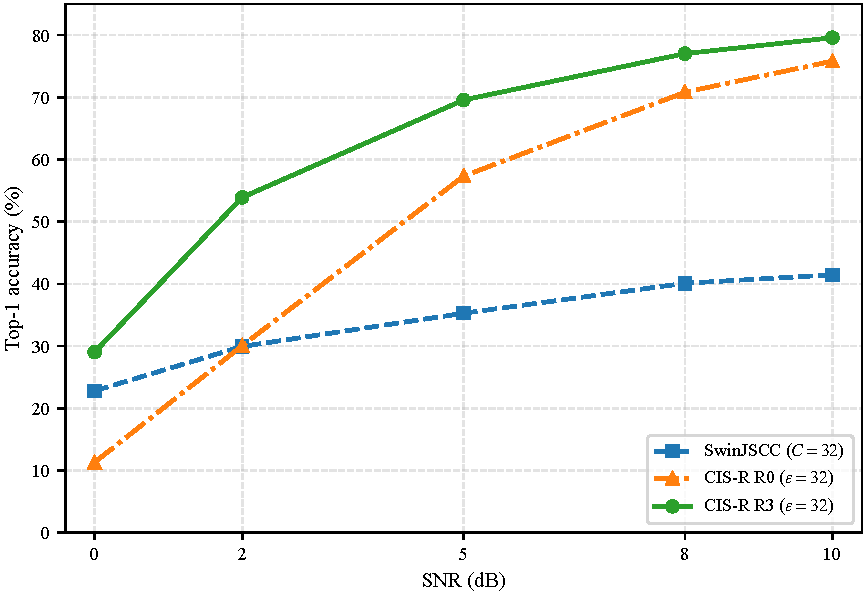
\includegraphics[width=0.86\linewidth]{figures/chapter6/figs/snr_accuracy_comparison_eps32.pdf}
    \bicaption{ImageNet-100 上不同信噪比下的 Top-1 分类准确率}{Top-1 classification accuracy versus SNR on ImageNet-100}
    \label{fig:ch6_snr_accuracy}
\end{figure}

\subsection{任务准确率与前向链路开销权衡}
\label{subsec:ch6_accuracy_cbr}

图~\ref{fig:ch6_accuracy_cbr} 绘制了不同单分块实值信道维数 $\epsilon$ 下 CIS-R 的逐轮准确率--CBR 轨迹，实验设置为 SNR $=5$~dB、$K=16$。当 $\epsilon=16$ 时，准确率由 R0 的 $19.66\%$ 提升至 R3 的 $40.28\%$，累计 CBR 从 $0.010417$ 增至 $0.012968$。当 $\epsilon=32$ 时，准确率由 $57.32\%$ 提升至 $69.56\%$，CBR 从 $0.020833$ 增至 $0.025935$。将 $\epsilon$ 增至 $64$ 后，基础轮准确率已达到 $77.64\%$，三轮增量重传后为 $81.44\%$，相应 CBR 从 $0.041667$ 增至 $0.051871$。

三种配置下，R0 至 R3 的准确率增益分别为 $20.62$、$12.24$ 和 $3.80$ 个百分点。基础轮通信预算越大，基础轮任务准确率越高，追加增量传输带来的增益也越小。在默认的 $\epsilon=32$ 配置下，三轮增量传输使累计 CBR 由 $0.020833$ 增至 $0.025935$，相较基础轮增加约 $24.5\%$，同时将 Top-1 分类准确率提高 $12.24$ 个百分点。该结果给出了轻量星上编码器通过增加前向链路开销换取任务性能的定量关系。图中 CBR 只统计前向链路开销，反馈比特未计入 CBR。

\begin{figure}[!htp]
    \centering
    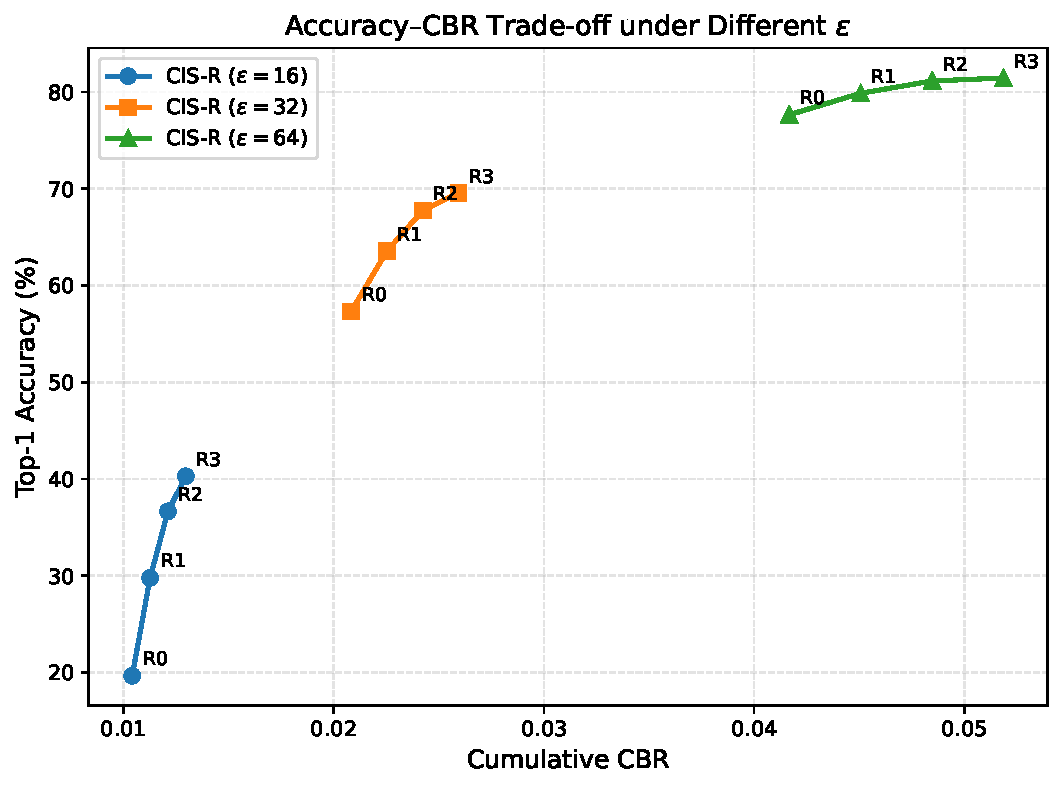
\includegraphics[width=0.86\linewidth]{figures/chapter6/figs/epsilon_accuracy_cbr_tradeoff.pdf}
    \bicaption{不同单分块信道维数下的任务准确率与 CBR 权衡}{Task accuracy--CBR trade-off under different per-patch channel dimensions}
    \label{fig:ch6_accuracy_cbr}
\end{figure}

\subsection{关键模块消融与反馈掩码分析}
\label{subsec:ch6_ablation_mask}

\noindent(1)~\textbf{关键模块消融}

图~\ref{fig:ch6_ablation_roundwise} 在 $\epsilon=32$、$K=16$ 和 SNR $=5$~dB 下比较 CIS-R 及其消融变体。各变体在同一轮次具有相同的名义 CBR，准确率差异由分块选择、反馈与轮次条件化特征变换以及接收端累积方式造成。完整 CIS-R 在 R3 达到 $69.56\%$。采用随机分块选择时，准确率降至 $66.64\%$。两者传输的符号数相同，$2.92$ 个百分点的差距来自分块选择策略。移除 SFT 后的 R3 准确率为 $68.58\%$，比完整方法低 $0.98$ 个百分点，表明基于二值反馈状态和轮次嵌入的 SFT 条件映射有助于生成补充表征。

接收端采用固定平均融合时，R3 准确率为 $68.24\%$。直接使用当前增量替换历史状态会在 R2 出现下降，最终仅达到 $62.00\%$，相较完整方法低 $7.56$ 个百分点。这一差距来自历史语义的丢失：跨轮累积需要保留已有状态中的有效信息，并根据当前增量调整融合比例。

\begin{figure}[!htp]
    \centering
    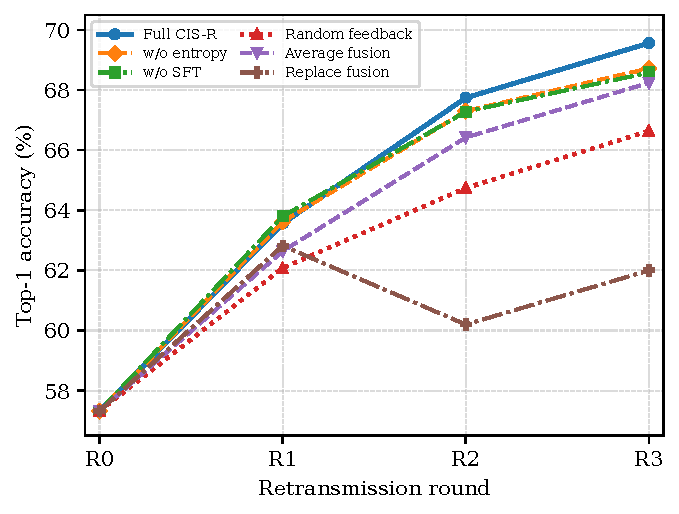
\includegraphics[width=0.88\linewidth]{figures/chapter6/figs/roundwise_ablation_nobits.pdf}
    \bicaption{CIS-R 关键模块的逐轮消融结果}{Round-wise ablation results of the key CIS-R modules}
    \label{fig:ch6_ablation_roundwise}
\end{figure}

\noindent(2)~\textbf{决策敏感反馈掩码分析}

图~\ref{fig:ch6_feedback_mask} 中的样例在 R0 分类错误，经过三轮增量重传后分类正确。地面接收端在 R0 后计算分块归因图，并生成 R1 的请求掩码。语义状态每更新一次，接收端都重新计算任务判决对各分块的敏感度，再确定下一轮掩码。因此，R1 至 R3 的选择区域随接收状态发生变化，并非重复请求首轮评分较高的分块。该样例给出了接收端依据当前任务判决调整增量传输位置的具体过程；分块选择策略的定量收益见图~\ref{fig:ch6_ablation_roundwise} 中的随机反馈对比。

\begin{figure}[!htp]
    \centering
    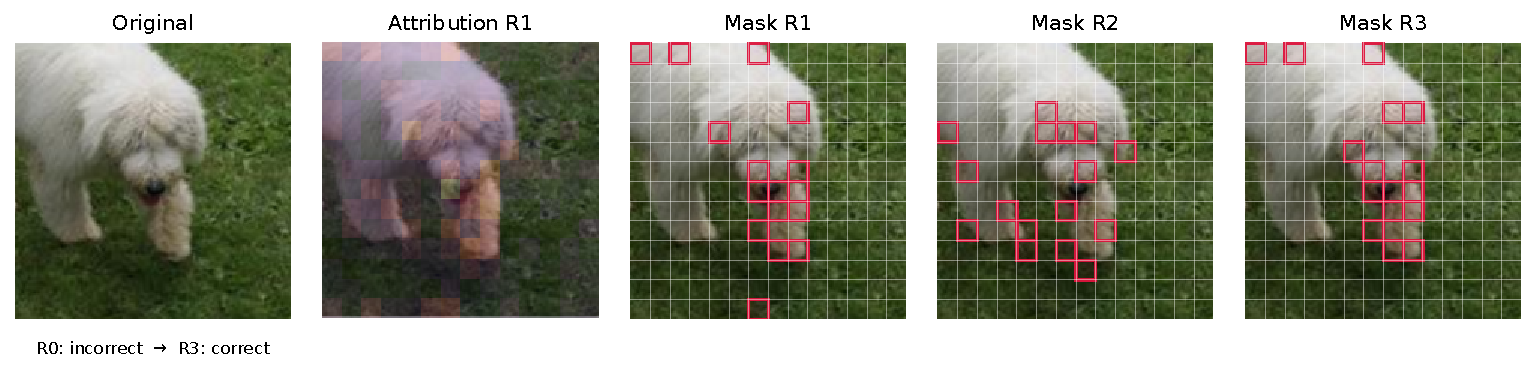
\includegraphics[width=\linewidth]{figures/chapter6/figs/feedback_mask_vis_paper.pdf}
    \bicaption{决策敏感分块归因与多轮反馈掩码}{Decision-sensitive patch attribution and multi-round feedback masks}
    \label{fig:ch6_feedback_mask}
\end{figure}

\subsection{分块选择数与增量重传轮数的影响}
\label{subsec:ch6_k_rounds}

\noindent(1)~\textbf{分块选择数的影响}

图~\ref{fig:ch6_k_sensitivity} 在 $\epsilon=32$、SNR $=5$~dB 下比较了 $K\in\{8,16,32\}$ 时的逐轮准确率和 R3 准确率--CBR 关系。三种配置的 R3 准确率分别为 $65.32\%$、$69.56\%$ 和 $73.10\%$，对应的累计 CBR 分别为 $0.023384$、$0.025935$ 和 $0.031037$。将 $K$ 从 $8$ 增至 $16$，增加 $0.002551$ 的 CBR 可获得 $4.24$ 个百分点的准确率增益；继续将 $K$ 从 $16$ 增至 $32$，附加 CBR 增加到前一阶段的两倍，但准确率增益降为 $3.54$ 个百分点。$K=16$ 在所测试配置中获得较高的准确率--CBR 增益比，后续实验采用该设置。反馈使用固定长度的分块位图，因此三种 $K$ 配置的每轮反馈量均为 $196$ bit。

\begin{figure}[!htp]
    \centering
    \begin{subfigure}[t]{0.48\linewidth}
        \centering
        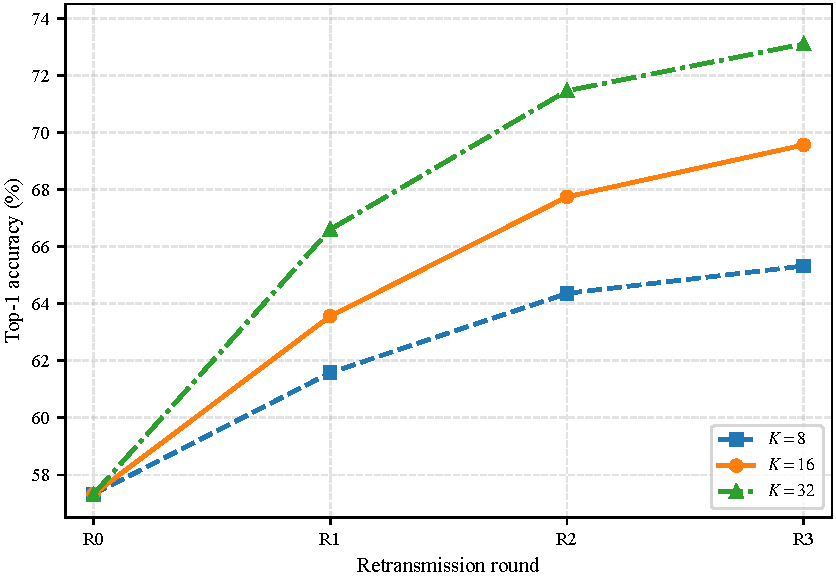
\includegraphics[width=\linewidth]{figures/chapter6/figs/k_sensitivity_roundwise.pdf}
        \caption{逐轮分类准确率}
        \label{fig:ch6_k_roundwise}
    \end{subfigure}
    \hfill
    \begin{subfigure}[t]{0.48\linewidth}
        \centering
        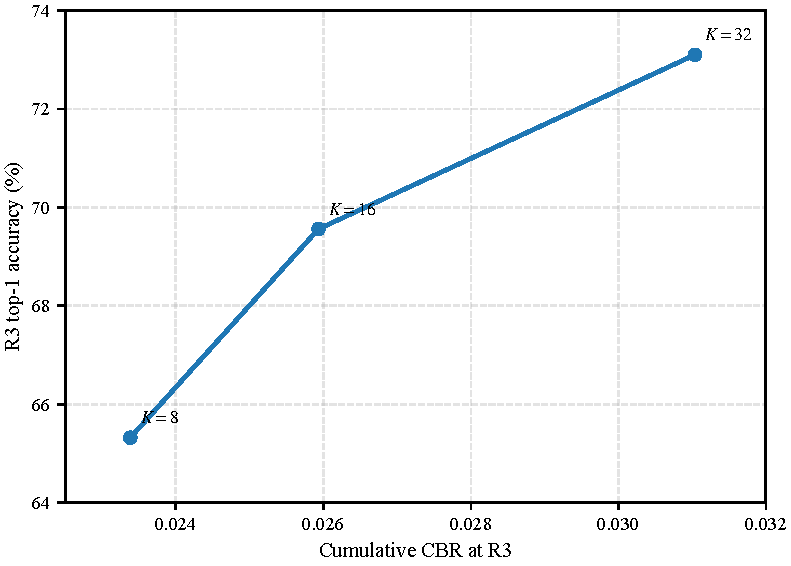
\includegraphics[width=\linewidth]{figures/chapter6/figs/k_sensitivity_accuracy_cbr.pdf}
        \caption{R3 准确率与累计 CBR}
        \label{fig:ch6_k_cbr}
    \end{subfigure}
    \bicaption{不同分块选择数下的任务准确率与前向链路开销}{Task accuracy and forward-link overhead under different numbers of selected patches}
    \label{fig:ch6_k_sensitivity}
\end{figure}

\noindent(2)~\textbf{增量重传轮数的影响}

图~\ref{fig:ch6_round_saturation} 考察继续增加重传轮次后的收益。实验在 $\epsilon=32$、$K=16$ 和 SNR $=5$~dB 下单独训练 $R_{\max}=6$ 模型，R0 至 R6 的准确率依次为 $57.32\%$、$63.96\%$、$67.90\%$、$69.32\%$、$70.56\%$、$71.04\%$ 和 $71.82\%$。从 R3 延长至 R6 只增加 $2.50$ 个百分点，CBR 却从 $0.025935$ 增至 $0.031037$，相对增加 $19.67\%$，同时多出三次反馈闭环。本文据此将 $R=3$ 作为默认设置。由于六轮模型单独训练，其 R3 准确率与默认三轮模型的 $69.56\%$ 略有差异。

\begin{figure}[!htp]
    \centering
    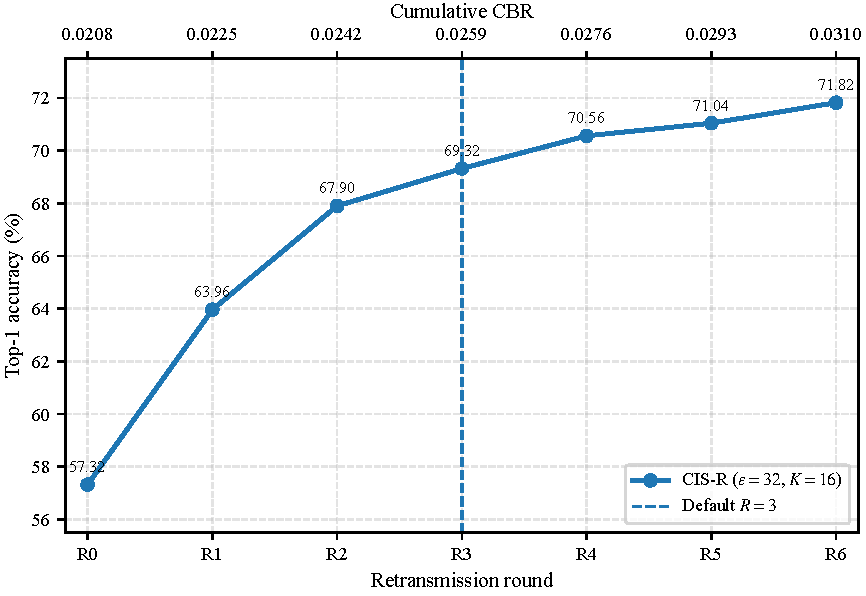
\includegraphics[width=0.86\linewidth]{figures/chapter6/figs/round_saturation_eps32_k16_snr5.pdf}
    \bicaption{增量重传轮数增加时的分类准确率饱和趋势}{Classification accuracy saturation with additional incremental retransmission rounds}
    \label{fig:ch6_round_saturation}
\end{figure}

\subsection{实现级模型开销与时变星地传输性能}
\label{subsec:ch6_deployment_trace}

\noindent(1)~\textbf{通信模型规模与 GPU 任务处理开销}

表~\ref{tab:ch6_complexity_latency} 按照第~\ref{subsec:ch6_setup}~节给出的硬件环境与统计口径，比较不同方法当前实现的端点模型规模、GPU 任务处理时延和峰值显存占用。其中，GPU 任务处理时延覆盖已实现的完整任务处理链路，但不包括符号传输、反馈传输和星地传播，因而不等同于端到端星地业务时延。对于无法从公开实现中明确拆分收发端的方法，仅报告通信模型总参数量。

\begin{table}[!htp]
    \centering
    \bicaption{不同方法当前实现的端点模型规模与 GPU 任务处理开销}{Endpoint model size and GPU task-processing cost of current implementations}
    \label{tab:ch6_complexity_latency}
    \small
    \renewcommand{\arraystretch}{1.15}
    \resizebox{\linewidth}{!}{
    \begin{tabular}{@{}lcccccc@{}}
        \toprule
        方法 & 输入尺寸 & 星上发送端参数量（M） & 地面接收端参数量（M） & 总参数量（M） & GPU 任务处理时延（ms） & 峰值显存（MiB） \\
        \midrule
        CIS-R（$\epsilon=64$，R3） & $224^2$ & $1.060$ & $1.214$ & $2.274$ & $45.340$ & $150.00$ \\
        SwinJSCC（$C=64$） & $224^2$ & $19.000$ & $14.064$ & $33.064$ & $16.347$ & $318.91$ \\
        Codebook（$C=80$） & $224^2$ & -- & -- & $519.940$ & $19.325$ & $2213.96$ \\
        DiffJSCC（$50$ 步） & $512^2$ & -- & -- & $5478.999$ & $4382.750$ & $22143.48$ \\
        \bottomrule
    \end{tabular}}
\end{table}

CIS-R 的星上发送端通信模型参数量为 $1.060$~M，地面接收端通信模型参数量为 $1.214$~M，总参数量为 $2.274$~M；星上仅部署分块映射、基础编码器和反馈条件化增量生成模块，任务模型推理与反馈计算均位于地面端。在表中所列当前实现与配置下，CIS-R 的通信模型总参数量和峰值显存占用最低。完整 R0--R3 GPU 任务处理时间为 $45.340$~ms，其中包含四次任务模型前向推理和三次基于梯度的反馈计算。SwinJSCC 和 Codebook 只执行单次前向处理，其 GPU 任务处理时延低于 CIS-R；DiffJSCC 的生成式恢复包含多次迭代，GPU 任务处理时延达到 $4382.750$~ms。上述结果用于说明 CIS-R 将较小的星上通信模型与计算量较高的地面任务处理相分离，不将不同输入尺寸、网络结构和交互轮数下的实现级结果解释为严格的同构复杂度比较。

\noindent(2)~\textbf{时变 LEO 星地传输性能}

时变星地链路仿真采用本地保存的双行根数（Two-Line Element，TLE）、卫星轨道几何与链路预算生成下行链路状态。仿真覆盖北京密云、喀什和三亚三个地面站，并在每个地面站的候选可见窗口中选取最长连续可见区间。轨迹驱动实验的轨道、链路预算、业务负载和通信配置如表~\ref{tab:ch6_trace_config} 所示。

\begin{table}[!htp]
    \centering
    \bicaption{轨迹驱动星地链路仿真配置}{Configuration of trace-driven satellite--ground link simulation}
    \label{tab:ch6_trace_config}
    \footnotesize
    \renewcommand{\arraystretch}{1.08}
    \begin{tabular}{@{}p{0.19\linewidth}p{0.74\linewidth}@{}}
        \toprule
        配置项 & 参数设置 \\
        \midrule
        轨道与可见窗口 & 本地保存的 $1584$ 颗 Starlink 卫星 TLE；轨迹时长 $900$~s，采样间隔 $0.1$~s；最低仰角 $40^\circ$；选取最长连续可见区间 \\
        地面站 & 北京密云（$40.3762^\circ$N，$116.8430^\circ$E）、喀什（$39.4704^\circ$N，$75.9898^\circ$E）和三亚（$18.3074^\circ$N，$109.3272^\circ$E），站点高度均设为 $0$~m \\
        卫星关联 & 从上升段候选卫星中选择当前仰角最小者，并保持关联直至其仰角低于 $40^\circ$ \\
        链路预算 & 载频 $f_c=20$~GHz，带宽 $B=400$~MHz，发送功率 $P_t=40$~dBm，收发天线总增益 $G_t+G_r=60$~dB，噪声功率谱密度 $N_0=-164$~dBm/Hz；采用自由空间路径损耗，附加衰减设为 $0$~dB \\
        参考链路 & 星地距离 $550$~km 时，自由空间路径损耗为 $173.27$~dB，接收功率为 $-73.27$~dBm，噪声功率为 $-77.98$~dBm，对应 SNR 为 $4.71$~dB \\
        业务与模型 & $500$ 幅 ImageNet-100 图像和 $500$ 幅 CIFAR-100 图像交替到达；共享星上发送端通信模型参数量为 $1.025$~M，两类数据分布对应的地面接收端通信模型参数量均为 $1.198$~M，均不包含下游任务模型 \\
        通信参数 & $\epsilon=32$，$K=16$，执行 R0--R3；每幅图像累计传输 $3904$ 个复信道符号，CBR 从 $0.020833$ 增至 $0.025935$，累计反馈 $588$~bit；前向链路符号速率为 $4\times10^8$ 复信道符号/s，反馈速率为 $1$~Mbit/s，单轮反馈周转时间为 $4$~ms \\
        \bottomrule
    \end{tabular}
\end{table}

时变星地链路实验采用第~\ref{subsec:ch6_setup}~节给出的两种图像分类数据分布。与表~\ref{tab:ch6_complexity_latency} 中 $\epsilon=64$ 的实现级开销测试不同，本实验采用 $\epsilon=32$，因此相应的星上发送端与地面接收端通信模型参数量分别为 $1.025$~M 和 $1.198$~M。两类图像共享同一个在 ImageNet-100 上训练并冻结的星上发送端，并分别使用对应的地面分类模型完成任务推理与反馈计算。北京密云、喀什和三亚的最长连续可见区间分别为 $322.0$、$649.3$ 和 $767.8$~s，对应 $3221$、$6494$ 和 $7679$ 个链路状态采样点，分别涉及 $4$、$6$ 和 $6$ 颗卫星。在每个增量轮开始时，仿真器读取当前 SNR 与星地斜距，依据当前 SNR 生成 AWGN，并利用斜距计算单向传播时延。任务驱动反馈和随机反馈使用相同的前向与反向负载，并对每幅图像、每个轮次采用相同的 AWGN 噪声样本；两种策略处理 $1000$ 幅图像时均传输 $3.904$~M 个前向复信道符号和 $588000$~bit 反馈信息，仿真不引入排队时延。

该实验直接使用在固定 SNR $=5$~dB 的 AWGN 信道下训练得到的 CIS-R 模型，在测试期间不重新训练模型，也不执行在线信道自适应。因此，实验用于考察固定信道条件下训练的 CIS-R 对所测试时变 SNR 轨迹的直接泛化性能，不用于推断其在未建模衰落、干扰或附加传播损耗条件下的性能。

为区分任务处理与星地通信时延，在 $\epsilon=32$ 的 R0--R3 配置下，分别测得 ImageNet-100 和 CIFAR-100 完整任务处理链路的 GPU 时延为 $49.10$~ms 和 $44.31$~ms，两类业务等权平均后记为 $T_{\mathrm{task}}^{\mathrm{case}}=46.704$~ms。平均端到端时延定义为
\begin{equation}\label{eq:ch6_e2e_latency}
T_{\mathrm{E2E}}^{\mathrm{avg}}
=T_{\mathrm{task}}^{\mathrm{case}}+T_{\mathrm{comm}}^{\mathrm{avg}},
\end{equation}
其中，$T_{\mathrm{comm}}$ 包括前向与反馈序列化时延、四次前向和三次反向单向传播时延，以及三次反馈周转时间。由于任务处理时延与通信时延分别测量，表~\ref{tab:ch6_trace_case} 报告二者均值之和，通信闭环时延的第 $95$ 百分位数在表后单独给出。

\begin{table}[!htp]
    \centering
    \bicaption{时变星地链路下的链路状态、端到端时延与分类准确率}{Link states, end-to-end latency, and classification accuracy over time-varying satellite--ground links}
    \label{tab:ch6_trace_case}
    \scriptsize
    \renewcommand{\arraystretch}{1.10}
    \resizebox{\linewidth}{!}{
    \begin{tabular}{@{}lccccccccc@{}}
        \toprule
        地面站 & 可见窗口（s） & SNR（dB） & 星地距离（km） & 仰角（$^\circ$） & 平均端到端时延（ms） & R0（\%） & 任务驱动 R3（\%） & 随机反馈 R3（\%） & 增益（百分点） \\
        \midrule
        北京密云 & $322.0$ & $1.29/3.22/5.29$ & $514.8/659.6/815.3$ & $40.0/54.0/81.3$ & $74.70$ & $50.6$ & $61.0$ & $55.6$ & $5.4$ \\
        喀什 & $649.3$ & $1.29/2.98/4.47$ & $565.6/673.8/815.6$ & $40.0/52.8/71.1$ & $75.03$ & $50.7$ & $61.1$ & $55.7$ & $5.4$ \\
        三亚 & $767.8$ & $1.41/3.71/5.65$ & $493.5/621.6/804.2$ & $40.0/55.9/85.6$ & $73.82$ & $56.5$ & $64.9$ & $60.4$ & $4.5$ \\
        \bottomrule
    \end{tabular}}
\end{table}

在前向和反馈负载完全相同的条件下，任务驱动反馈相较随机反馈在北京密云、喀什和三亚链路上分别提高 $5.4$、$5.4$ 和 $4.5$ 个百分点。三个站点的平均通信闭环时延及其第 $95$ 百分位数分别为 $28.00/31.08$、$28.33/30.75$ 和 $27.11/29.93$~ms。前向负载与反馈信息的序列化时延分别为 $0.00976$~ms 和 $0.588$~ms，通信闭环时延主要由多次星地传播和三次反馈周转构成。在所测试的轨迹、链路预算和固定信道训练设置下，基于当前任务判决敏感度的分块优先级在 SNR、星地距离和仰角随可见窗口变化时仍取得了高于随机反馈的平均分类准确率。该实验还表明，在保持星上发送参数不变的条件下，通过地面接收端适配可以支持新的图像分类数据分布；该结论不扩展至分类、检测和分割等不同任务类型之间的迁移。

\section{本章小结}

本章面向星上发送端与地面接收端资源和任务功能非对称的 LEO 图像传输场景，提出接收端驱动的 CIS-R 闭环语义重传机制。地面接收端根据当前任务判决生成分块级反馈，星上发送端依据反馈掩码完成候选增量生成与选择性传输，地面接收端通过掩码引导的门控累积融合当前增量与历史分块表征，并基于更新后的状态继续生成下一轮反馈。在线传输阶段，星上发送端无需部署或访问下游任务模型，任务模型推理、分块优先级计算与反馈生成均部署在地面端，从而在不扩展当前星上通信模型规模的条件下利用多轮选择性增量通信提高地面任务性能。

在 ImageNet-100 高压缩率图像传输实验中，三轮增量传输以约 $24.5\%$ 的累计 CBR 增幅换取 $12.24$ 个百分点的 Top-1 分类准确率增益，消融实验同时验证了任务驱动反馈、反馈与轮次条件化特征变换及自适应跨轮累积的作用。在当前 $\epsilon=64$ 的实现级配置下，星上发送端与地面接收端通信模型参数量分别为 $1.060$~M 和 $1.214$~M，总参数量为 $2.274$~M，约为所测 DiffJSCC 生成式实现的 $1/2400$；该对比仅适用于当前输入尺寸、迭代次数和实现流程。在轨迹驱动星地链路仿真中，任务驱动反馈较随机反馈在北京密云、喀什和三亚三个可见窗口内分别提高 $5.4$、$5.4$ 和 $4.5$ 个百分点的平均分类准确率，平均端到端时延为 $73.82$--$75.03$~ms。上述结论限定于所测试的 TLE 轨迹、自由空间链路预算、AWGN 和固定信道训练设置，不扩展至未建模的传播条件或不同任务类型之间的迁移。
